\model{Branching and Merging}
  \begin{center}
    \begin{tabular}{p{2.5in}p{2.5in}}
      \begin{minipage}{2.5in}
        \centering
        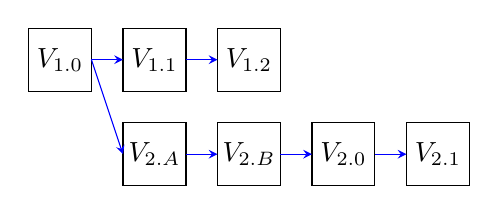
\begin{tikzpicture}[scale=0.8]    
          \draw (0,0) rectangle (1,1);
          \node at (0.5,0.5) {$V_{1.0}$};
          \draw (1.5,0) rectangle (2.5,1);
          \node at (2,0.5) {$V_{1.1}$};
          \draw (3,0) rectangle (4,1);
          \node at (3.5,0.5) {$V_{1.2}$};
          \draw (1.5,-0.5) rectangle (2.5,-1.5);
          \node at (2,-1) {$V_{2.A}$};
          \draw (3,-0.5) rectangle (4,-1.5);
          \node at (3.5,-1) {$V_{2.B}$};
          \draw (4.5,-0.5) rectangle (5.5,-1.5);
          \node at (5,-1) {$V_{2.0}$};
          \draw (6,-0.5) rectangle (7,-1.5);
          \node at (6.5,-1) {$V_{2.1}$};      
          \draw[blue,-stealth] (1,0.5) -- (1.5,0.5);
          \draw[blue,-stealth] (1,0.5) -- (1.5,-1);
          \draw[blue,-stealth] (2.5,0.5) -- (3,0.5);
          \draw[blue,-stealth] (2.5,-1) -- (3,-1);
          \draw[blue,-stealth] (4,-1) -- (4.5,-1);
          \draw[blue,-stealth] (5.5,-1) -- (6,-1);
        \end{tikzpicture}\par
        Scenario \#1
      \end{minipage}
      &
      \begin{minipage}{2.5in}
        \centering
        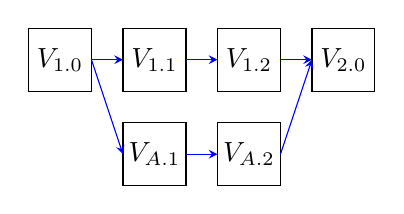
\begin{tikzpicture}[scale=0.8]    
          \draw (0,0) rectangle (1,1);
          \node at (0.5,0.5) {$V_{1.0}$};
          \draw (1.5,0) rectangle (2.5,1);
          \node at (2,0.5) {$V_{1.1}$};
          \draw (3,0) rectangle (4,1);
          \node at (3.5,0.5) {$V_{1.2}$};
          \draw (4.5,0) rectangle (5.5,1);
          \node at (5,0.5) {$V_{2.0}$};
          \draw (1.5,-0.5) rectangle (2.5,-1.5);
          \node at (2,-1) {$V_{A.1}$};
          \draw (3,-0.5) rectangle (4,-1.5);
          \node at (3.5,-1) {$V_{A.2}$};
          \draw[blue,-stealth] (1,0.5) -- (1.5,0.5);
          \draw[blue,-stealth] (2.5,0.5) -- (3,0.5);
          \draw[blue,-stealth] (4,0.5) -- (4.5,0.5);
          \draw[blue,-stealth] (1,0.5) -- (1.5,-1);
          \draw[blue,-stealth] (2.5,-1) -- (3,-1);
          \draw[blue,-stealth] (4,-1) -- (4.5,0.5);
        \end{tikzpicture}\par
        Scenario \#2
      \end{minipage}
    \end{tabular}
  \end{center}
  
  {\it\large Refer to Model 2 above as your team develops consensus answers
    to the questions below.}

  \quest{25 min}
    
  \Q After an initial version of a program is finished,
    you may wish to start working on new features without breaking
    the existing version. Versions that have not yet been released 
    are sometimes labeled with the names alpha and beta. 
    You may then continue to make small bug fixes
    to the existing version in parallel with the major changes
    being made to the new version.  These parallel versions of the
    software are called {\it branches} and creating a new parallel
    version is called {\it branching}.
    \begin{enumerate}
      \item Identify the initial version of the repository
        shown in scenario \#1 of the model along with the versions
        that are bug fixes of that initial version.
        \begin{answer}[0.75in]
          {$V_{1.0}$}, {$V_{1.1}$}, and {$V_{1.2}$}
        \end{answer}

      \item How are versions {$V_{1.0}$} and {$V_{2.A}$} of this first scenario related?
        \begin{answer}[0.5in]
          They are essentially the same; {$V_{2.A}$} is a copy of {$V_{1.0}$} 
          to which no changes have yet been applied.
        \end{answer}

      \item How are versions {$V_{1.2}$} and {$V_{2.0}$} related?
        \begin{answer}[0.5in]
          They share a common ancestor, {$V_{1.0}$}, but have had a 
          separate set of edits applied.
        \end{answer}

      \item Create a timeline diagram starting with scenario \#1 of the model
        and showing the following additional actions.
        \begin{center}
          \begin{minipage}{4.5in}
            \begin{enumerate}[i.]
              \itemsep -2pt
              \item A new release is added to the $V_1$ branch
              \item A new release is added to the $V_2$ branch
              \item A new branch with versions $3.A$, $3.B$, and
                $3.0$ is added.
            \end{enumerate}
          \end{minipage}
        \end{center}
        \begin{answer}[1.5in]
          Answers will vary
        \end{answer}
    \end{enumerate}
    
  \Q When multiple people are working on the same repository, it
    is common practice for a group of them to create a branch in
    which to add and test their code and then {\it merge} that branch
    back into the main branch (called the {\it trunk}) when they
    are done.  An example of this is shown in scenario \#2.
    \begin{enumerate}
      \item Why might a development team choose to add new
        features in a branch instead of in the trunk?
        \begin{answer}[1in]
          So they can take advantage of version control features 
          (such as saving intermediate versions, comparing edits, 
          sharing edits, reverting edits), without impacting the 
          trunk.
        \end{answer}

      \item What challenges might the programmers face when
        merging their branch back into the trunk?  How could these
        challenges be minimized?
        \begin{answer}[1in]
          Bug fixes in the trunk may need to be made to the branch 
          as well. The trunk changes should be merged to the branch 
          regularly.
        \end{answer}

      \item Draw a timeline diagram starting with scenario \#2 of 
        the model that shows another team
        working on the same project creating branch $B$ based on
        version $1.1$ of the trunk, creating versions $B.1$
        and $B.2$, and then merging it into version 2.0.
        \begin{answer}[1.6in]
          Answers will vary
        \end{answer}
    \end{enumerate}
    
  \Q Add nodes and/or arrows to the diagram below to create a
    timeline diagram for\key\\[-2.5mm] each of the following sequence of events.
    \begin{center}
      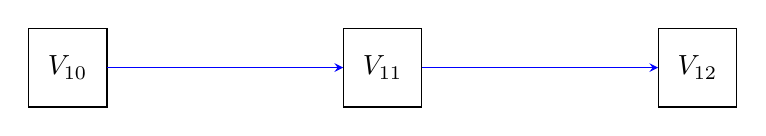
\begin{tikzpicture}[scale=1]
        \draw (0,0) rectangle (1,1);
        \node at (0.5,0.5) {$V_{10}$};
        \draw (4,0) rectangle (5,1);
        \node at (4.5,0.5) {$V_{11}$};
        \draw (8,0) rectangle (9,1);
        \node at (8.5,0.5) {$V_{12}$};
        \draw[blue,-stealth] (1,0.5) -- (4,0.5);
        \draw[blue,-stealth] (5,0.5) -- (8,0.5);
      \end{tikzpicture}
    \end{center}
    \begin{enumerate}
      \item Version 10 is finished and version 11 is in
        progress, but defects in version 10 must be fixed and
        released (as version $10.A$) before version 11 is
        ready. 
        \begin{answer}[1in]
        \end{answer}

      \item Version $10.A$ is merged into the main branch before
        version 11 is released.
        \begin{answer}[1in]
        \end{answer}

      \item Version 11 is completed and version 12 is in progress,
        but some developers are exploring a different approach to
        error handling (version $11.A$), which might be included in
        version 12, but might also be delayed until version 13.
        \begin{answer}[1in]
        \end{answer}

      \item The two developers working on version $11.A$ disagree
        on how best to proceed.  One finishes a smaller set of 
        changes (as version $11.B$) that are added before version
        12 is finished.  The other continues with a larger set of
        changes, now called version $11.C$, that will be added to
        version 13.
        \begin{answer}[1in]
        \end{answer}
    \end{enumerate}
    
  \Q What seems harder, technically -- branching or merging?
    Explain why.
    \begin{answer}[1in]
      Branching is simply making a copy; easy! 
      Merging requires comparison of changes made to two sources; hard!
    \end{answer}

  \Q One popular modern version control system is called 
    {\tt Git}. Because {\tt Git} is a {\it distributed} VCS, it
    it uses slightly different terminology from that developed above.
    Conduct some internet searches to determine the {\tt git} commands
    that would accomplish each of the following.
    \begin{enumerate}
      \itemsep 10pt
      \item Initialize a new repository
        \hfill\ans[2.25in]{git init {\it project-name }}

      \item Create a local copy of a remote repository
        \hfill\ans[2.25in]{git init {\it project-url }}

      \item Check the status of the files in your local repository
        \hfill\ans[2.25in]{git status}

      \item Add files to your local repository
        \hfill\ans[2.25in]{git add {\it files}}

      \item Commit changes to your local repository
        \hfill\ans[2.25in]{git commit -m {\it message}}

      \item Update your local repository from a remote repository
        \hfill\ans[2.25in]{git pull}

      \item Send your local changes to the remote repository
        \hfill\ans[2.25in]{git push}

      \item Create a new branch in your local repository  
        \hfill\ans[2.25in]{git branch {\it branch-name}}
    \end{enumerate}